\chapter*{Forward}
\begin{figure}[t!]
    \centering
    \subfigure[Cartoon 2]{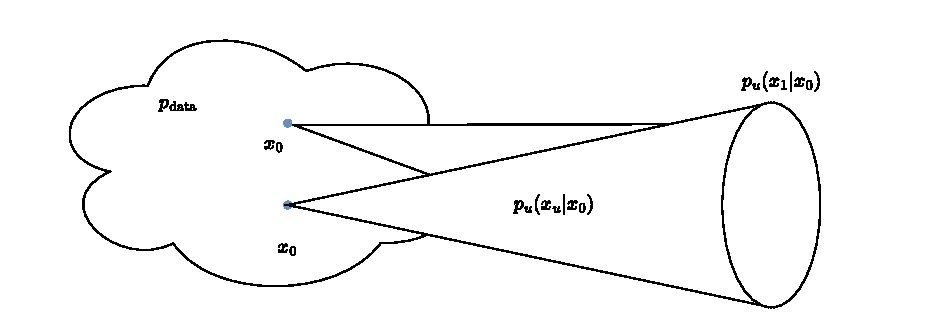
\includegraphics[width=0.3\linewidth]{plots/cartoon-2.pdf}\label{fig:cartoon2}}
    \hfill
    \subfigure[Cartoon 3]{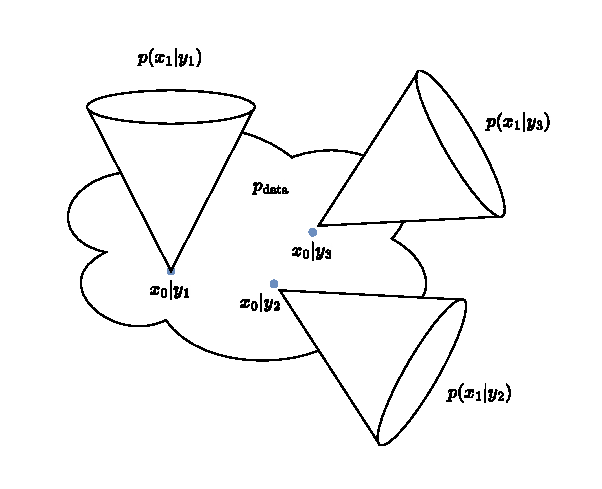
\includegraphics[width=0.3\linewidth]{plots/cartoon-3.pdf}\label{fig:cartoon3}}
    \hfill
    \subfigure[Cartoon 4]{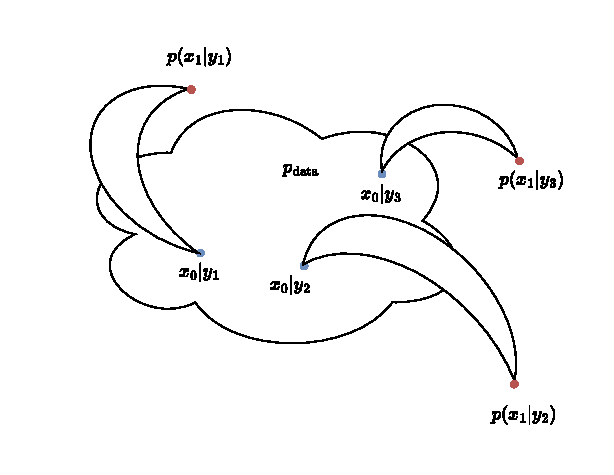
\includegraphics[width=0.3\linewidth]{plots/cartoon-4.pdf}\label{fig:cartoon4}}
    \caption{Cartoons 2--4.}
    \label{fig:cartoons2to4}
\end{figure}

Part I explores continuous-depth models, including score-based generative models, Schr\"odinger bridges, and flow-matching models. Score-based models use SDEs to connect a data distribution to a tractable reference distribution through diffusion. Schr\"odinger bridges can connect prescribed endpoint distributions; flow-matching methods can be formulated for a range of prescribed probability paths.

Some methods provide \textit{simulation-free} objectives for training continuous normalising flows (CNFs), avoiding a black-box ODE solve at every training step. Likelihood evaluation and sampling can still require numerical ODE integration. The first example considered here is included in \chapref{ch:diffusion}.

For models that define a normalised density, likelihoods can be evaluated and used to study model behaviour, although likelihood alone does not diagnose generalisation errors. \Chapref{ch:ll} presents experiments involving likelihood, including whether a model distinguishes an image of a red ball paired with the correct caption from one paired with ``blue cube''.

Schr\"odinger bridges (SBs) and conditional flow matching (CFM) are related design choices, not mutually exclusive methods. SBs define a stochastic reference process and seek a path close to it under endpoint constraints; flow matching trains a vector field against a chosen probability path. A path need not be optimal transport unless the construction imposes that property. Stochasticity can act as an entropic regulariser, while excessive input variance may make training harder. The methods are outlined in \chapref{ch:cfm} and evaluated in \chapref{ch:cfmse}.

An additional investigation on SBs and CFMs concerns their ability to directly predict data from an input sample. This removes the continuous-depth aspect to these models, and introduces similarities to curriculum learning and data augmentation. A typical simulation-free objective for SB and CFM involves predicting a data sample given a sample from the probability path. If by this training the end-to-end data prediction is accurate, then the advantage of continuous-depth may not be increased capacity but instead through improved parameter optimisation.

This thesis makes an important distinction of the variable $u$. In the literature it is common to use $t$ to denote depth as this is consistent with the differential equations literature. The use of $t$ for depth becomes problematic in this thesis as the concept of time is better suited to the time-progression of a series, as is later described in part II. As a result, $u$ is used in part I to represent the level of depth through the DE, and $t$ is used to represent time within a series.



